\documentclass{emulateapj}
\submitted{{\it Submitted for publication in ApJ}}
\usepackage{multirow,color,wrapfig,ulem}
\usepackage {graphicx}
\usepackage{graphics}
\usepackage[dvips]{epsfig}
\bibliographystyle{apj}
\newcommand{\jcap}{JCAP}
\newcommand{\avg}[1]{\langle{#1}\rangle}
\newcommand{\nscatt}{\langle N_{\rm  scatt}\rangle}
\newcommand{\ly}{{\ifmmode{{\rm Ly}\alpha~}\else{Ly$\alpha$~}\fi}}
\newcommand{\hMpc}{{\ifmmode{h^{-1}{\rm Mpc}}\else{$h^{-1}$Mpc }\fi}}
\newcommand{\hGpc}{{\ifmmode{h^{-1}{\rm Gpc}}\else{$h^{-1}$Gpc }\fi}}
\newcommand{\hmpc}{{\ifmmode{h^{-1}{\rm Mpc}}\else{$h^{-1}$Mpc }\fi}}
\newcommand{\hkpc}{{\ifmmode{h^{-1}{\rm kpc}}\else{$h^{-1}$kpc }\fi}}
\newcommand{\hMsun}{{\ifmmode{h^{-1}{\rm
        {M_{\odot}}}}\else{$h^{-1}{\rm{M_{\odot}}}$}\fi}}
\newcommand{\hmsun}{{\ifmmode{h^{-1}{\rm
        {M_{\odot}}}}\else{$h^{-1}{\rm{M_{\odot}}}$}\fi}}
\newcommand{\Msun}{{\ifmmode{{\rm {M_{\odot}}}}\else{${\rm{M_{\odot}}}$}\fi}}
\newcommand{\msun}{{\ifmmode{{\rm {M_{\odot}}}}\else{${\rm{M_{\odot}}}$}\fi}}
\newcommand{\lya}{{Lyman $\alpha$~}}
\newcommand{\clara}{{\texttt{CLARA}}~}
\newcommand{\rand}{{\ifmmode{{\mathcal{R}}}\else{${\mathcal{R}}$ }\fi}}
\newcommand{\hs}{{\hspace{1mm}}}
\newcommand{\kms}{{\ifmmode{{\mathrm{\,km\ s}^{-1}}}\else{\,km~s$^{-1}$}\fi}}
% definition to produce a "less than or similar to" symbol
\def\lsim{~\rlap{$<$}{\lower 1.0ex\hbox{$\sim$}}}
% definition to produce a "greater than or similar to" symbol
\def\gsim{~\rlap{$>$}{\lower 1.0ex\hbox{$\sim$}}}
%@arxiver{fig3.pdf,fig11a.pdf, fig11b.pdf}
\begin{document}

\title{A new method to estimate dark matter halo concentrations}
\shorttitle{New method to estimate concentrations}

\shortauthors{Poveda \& Forero-Romero}

\author{Christian Poveda, Jaime E. Forero-Romero}
\affil{Departamento de F\'{i}sica, Universidad de los Andes, Cra. 1
No. 18A-10, Edificio Ip, Bogot\'a, Colombia}
\email{cn.poveda542@uniandes.edu.co}
\email{je.forero@uniandes.edu.co}
\author{Juan Carlos Mu\~noz-Cuartas}
\affil{UdeA, Medell\'in, Colombia}
\email{xxx@udea.edu.co}


\keywords{ methods: numerical --- galaxies: halos --- cosmology: theory --- dark
matter}
\begin{abstract}

We present a new method to estimate the concentration of dark matter
halos in N-body simulations.
Our method is based on a fit to the integrated mass profile as a function of
halo radius.
The main advantage of this method is that it uses the full particle information
without any binning.
We test our method both on mock and N-body halos to compare it against
two popular methods to find concentrations: maximum radial velocity
measurements and radial particle binning to estimate the density.
Tests on the mock halos show that the accuracy of our method to
recover input concentrations varies with the number of particles in
the halo. For halos sampled with $20$ particles our method recovers
the input concentration with $10\%$ accuracy, while for the maximum
radial velocity and density methods the accuracy is on the order of $20\%$ and
$100\%$, respectively. For halos samples with $10^4$ particles our
method achieves an accuracy of $0.01\%$ while the velocity and density
methods achieve $0.1\%$ and $1\%$ accuracy, respectively.
We also measure the mass-concentration relationship on the N-body
data.
With respect to the other two approaches our method produces a
flatter relationship, while its normalization falls below the maximum
velocity method and above the density method.
\end{abstract}



\section{Introduction}
\label{sec:introduction}
In the concordance cosmology paradigm the matter content of the
Universe is dominated by dark matter, a collisionless fluid shaped by
gravitational interactions.
Simulations of dark matter dominated universes during the last three
decades have provided valuable insights into the large scale structure
formation process, showing a remarkable success when theoretical
results are compared against observations of the galaxy distribution
obtained from large surveys.
\citep{Springel2005,2011ApJ...740..102K}.

On galactic scales the most striking results of these simulations is
that dark matter overdensities closely follow a universal density
profile. 
In a first approximation this profile is spherically symmetric and its
density only dependens on the radial coordinate.
The universality of this profiles seems to be independent of the
cosmological parameters and is self-similar for different spatial
scales after an adequate re-scaling is applied. 
\citep{NFW,Taylor2001}

One the most popular parameterization for a dark matter halo radial density
distribution is the Navarro-Frenk-White (NFW) profile
\citep{NFW}.
This profile is a double power law in radius, where the transition break
happens at the so-called scale radius $r_s$.
The ratio between the scale radius and the virial radius $R_v$, which
defines a natural scale for the halo, is known as the concentration
$c=R_v/r_s$. 
Simulations show that the concentration is a strong function of halo mass and
redshift. 

%%%

High resolution simulations of Milky Way sized dark matter halos
\citep{Navarro2010} show that the universality property is not
perfect and that a better fitting parameterization to the radial
density profile is provided by the Einasto profile
\citep{Einasto1965}.
However, the NFW density profile and its concentration have become a
standard metric to describe the structure of dark matter
halos.


Observationally, the relationship between halo mass and concentration
could provide a potential test of LCDM on galactic scales.
For this motivation a great deal of effort has been
invested in calibrating this relationship with simulations
\citep{Neto2007,Duffy2008,Munoz2011,Prada2012,Ludlow2014} and 
finding the best possible way to constraint it with observations
\citep{Buote2007,Comerford2007,Mandelbaum2008,Giocoli2014,Foex2014,Shan2015}.

From the computational point of view there are two main methods to
estimate the concentration parameter of a dark matter halo in a N-body
simulation.
The first method takes the particles composing the halos
and bins them in logarithmic radii to estimate the density in each
bin, then it proceeds with a fit of this density estimation as a
function of the radius.
A second method uses an analytic property of the
NFW that relates the maximum of the ratio of the circular velocity to
the virial velocity.
The concentration can be then found as the root of an algorithmnic
equation dependent on this maximum value.

The first method is straightforward to apply but presents two
disadvantages.
First, it requires a large number of particles in
order to have a proper density estimate in each bin.
This makes the method robust only for halos with at least  $10^3$
particles.
The second problem is that there is not a way to estimate the optimal
bin size, different choices produce different results for the
concentration.

The second method solves the two problems mentioned above.
It works with low particles numbers and does not involve data
binning.
However, it effectively takes into account only a single data point
and discards the behaviour of the ratio $V_{\rm circ}/V_{\rm vir}$ below and
above its maxima.
Additionally, small fluctuations on the value of this maximum can
yield large perturbations on the estimated concentration parameter.

In this paper we propose a new method to estimate the dark matter halo
concentration in halos obtained in numerical simulations.
It builds the cumulative mass profile from the particle data in the
N-body simulation to find the best possible concentration value using
a Markov Chain Monte Carlo (MCMC) methodology.


Our proposal has two advantages with respect to the two methods mentioned
above. 
It does not involve data binning and does not throw away data points.
Furthermore, the MCMC approach allows for an straightforward
estimation of the uncertainties in the concentration parameter, and
inclusion of informative priors.

%%%

\section{Basic properties of the NFW density profile}
\label{sec:basics}

\begin{figure*}
\begin{center}
  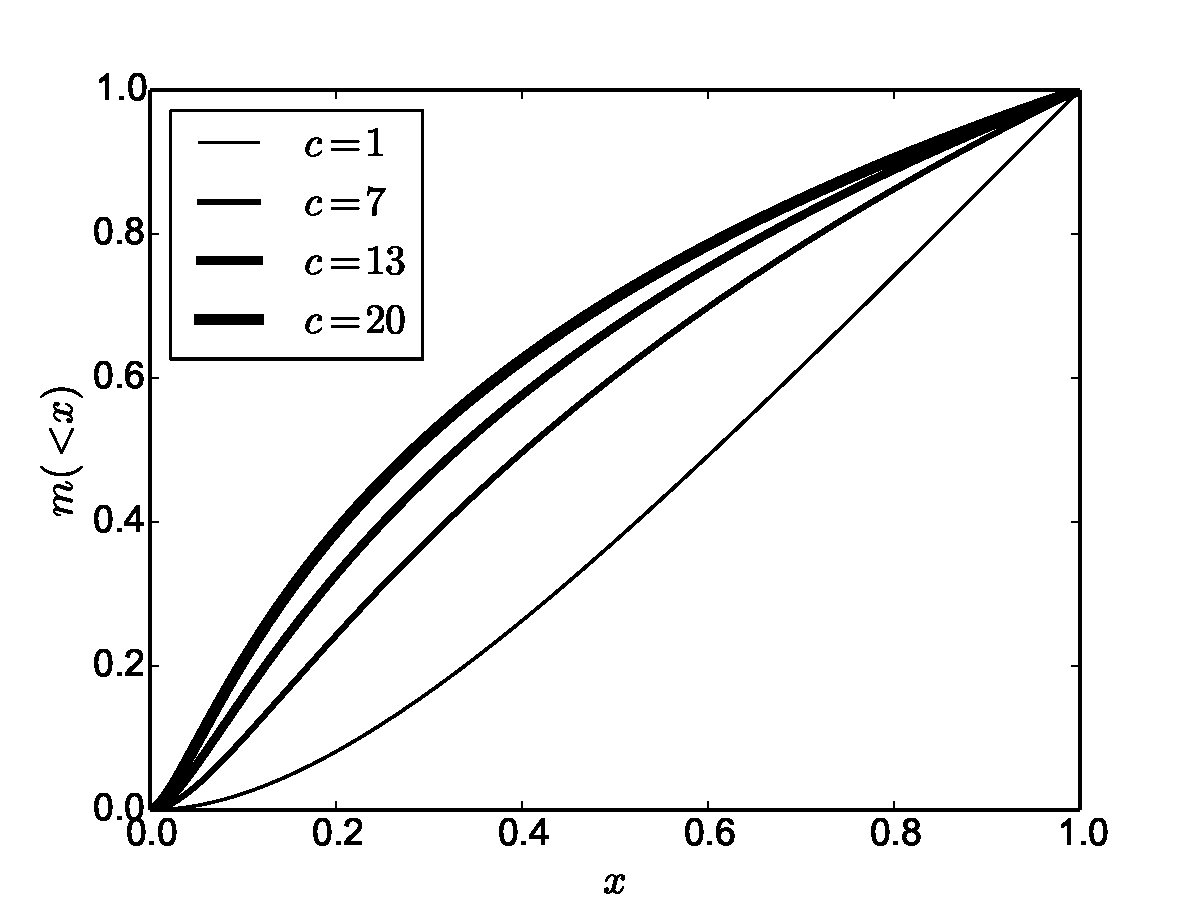
\includegraphics[width=0.48\textwidth]{nfw_normalized.pdf}
  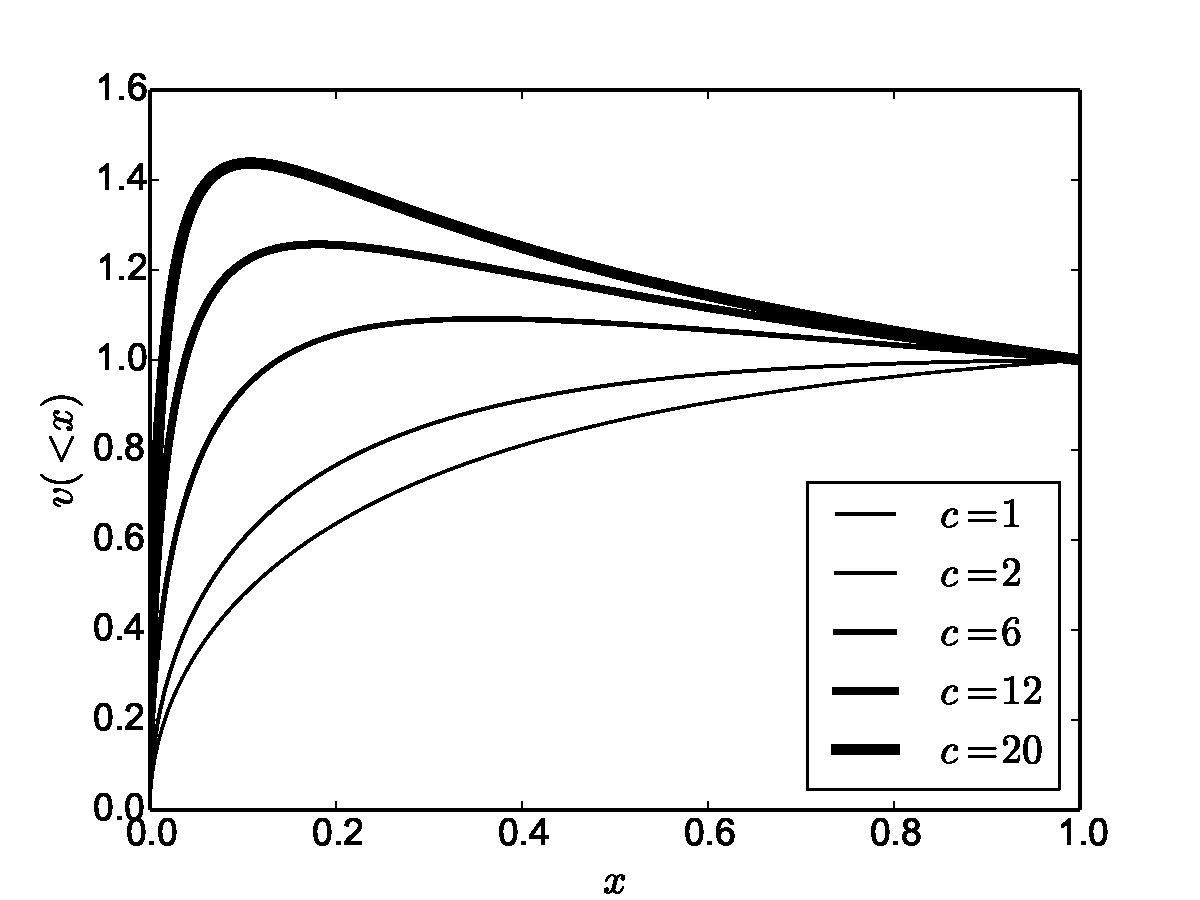
\includegraphics[width=0.48\textwidth]{vel_normalized.pdf}
\end{center}
\caption{Dimensionless mass (left) and velocity (right) profiles as a
  function of the dimensionless radius for different concentration
  values. \label{fig:profiles}}
\end{figure*}

\begin{figure*}
\begin{center}
  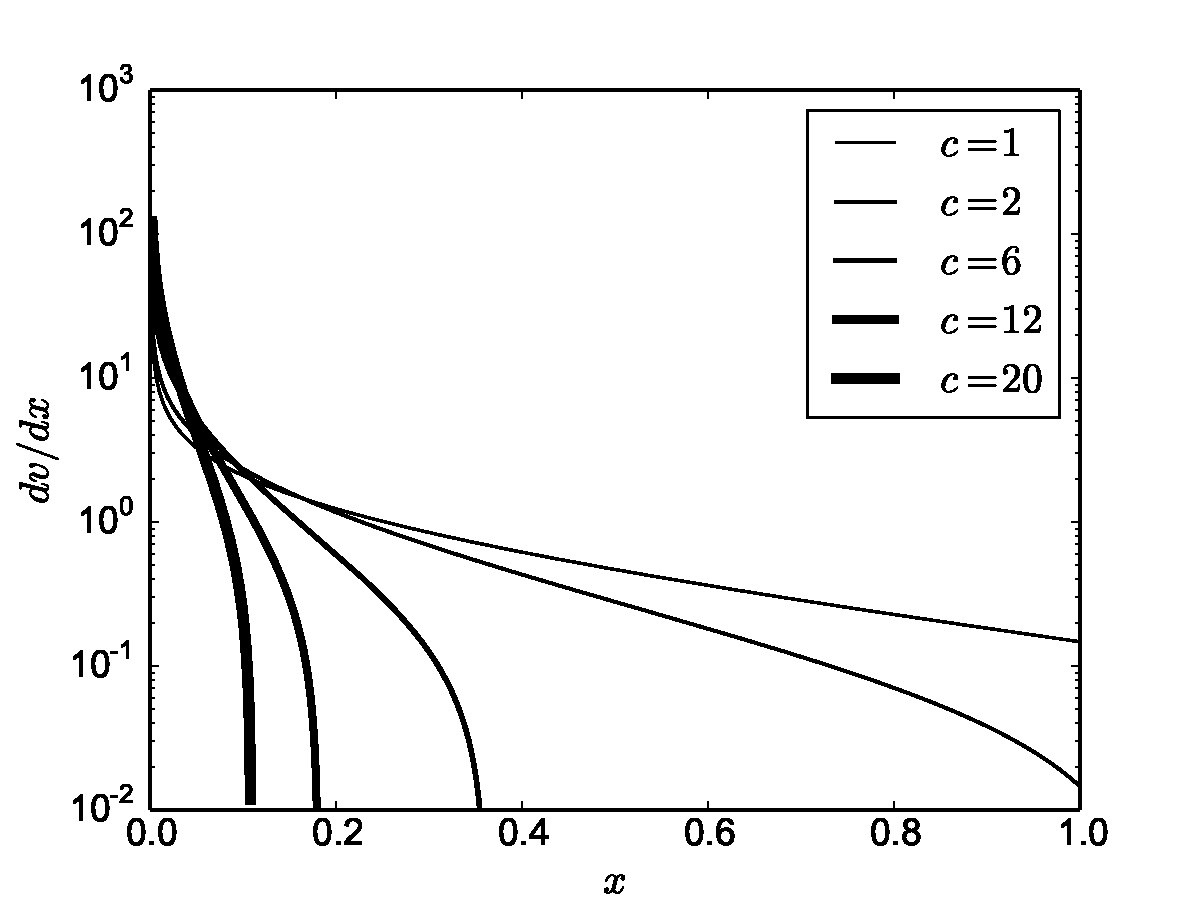
\includegraphics[width=0.48\textwidth]{dv_dx.pdf}
  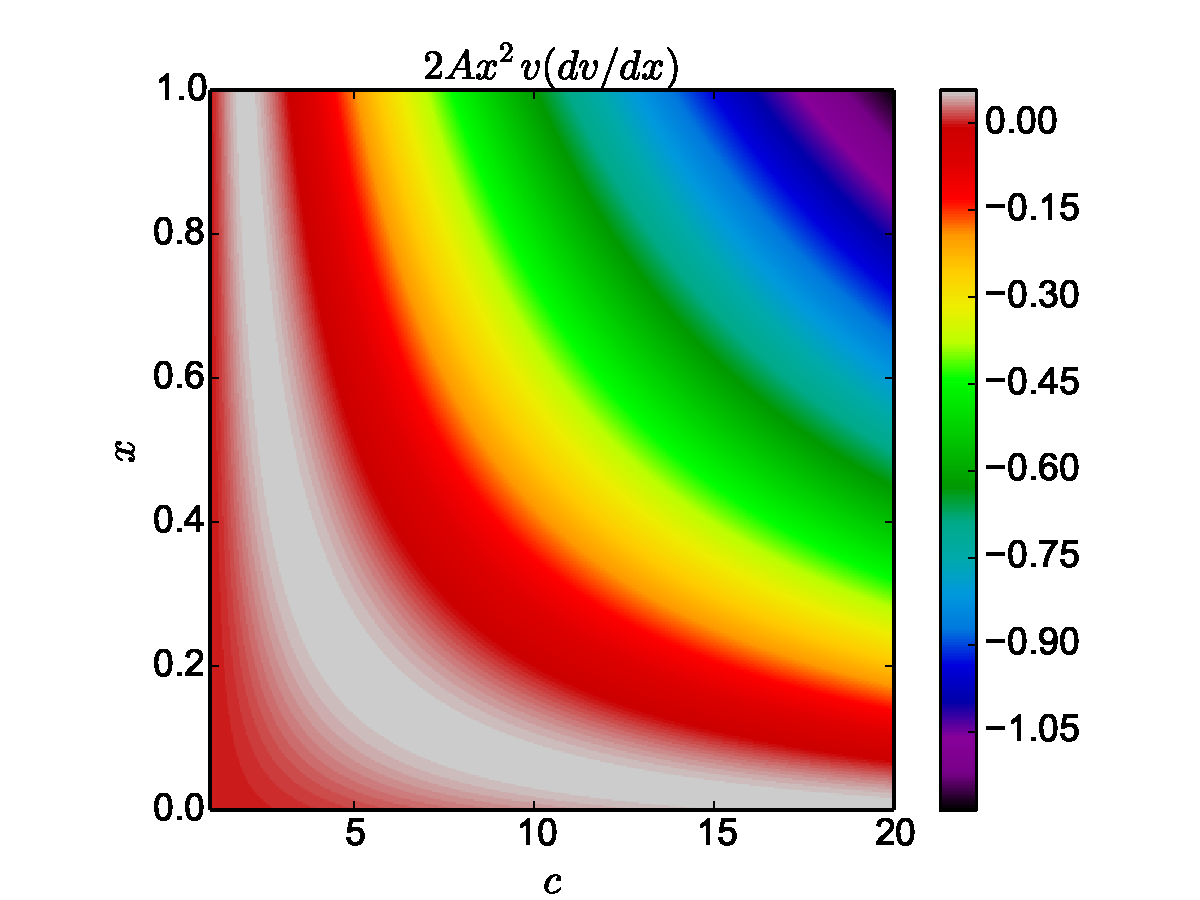
\includegraphics[width=0.48\textwidth]{zeros.pdf}
\end{center}
\caption{Dimensionless derivative of the velocity profile as a
  function of the dimensionless radius for different concentration
  values. \label{fig:profiles}}
\end{figure*}

\subsection{Density profile}

The NFW density profile can be written as

\begin{equation}
\rho(r) = \frac{\rho_c\delta_c}{r/r_s(1+r/r_s)^2},
\label{eq:definition}
\end{equation}
%
where $\rho_c\equiv 3H^2/8\pi G$ is the Universe critical density,
$\delta_c$ is the halo dimensionless characteristic density and $r_s$
is the scale radius. This radius marks the transition
between the power law scaling $\rho\propto r^{-1}$ for
$r<r_s$ and $\rho\propto r^{-3}$ for  $r>r_s$.

We define the virial radius of a halo, $r_v$, as the boundary of the
spherical volume that encloses a density of $\Delta_h$ times
the average density of the Universe. 
The corresponding mass $M_{v}$, the virial mass, can be written as
$M_{v} = \frac{4\pi}{3}\bar{\rho}\Delta_h r_v^3$.


\subsection{Integrated Mass}
From these definitions we can compute the total mass enclosed inside a
radius $r$:
\begin{equation}
M(<r) = 4\pi\rho_c\delta_c  r_s^3\left[\ln \left
  (\frac{r_s+r}{r_s}\right) - \frac{r}{r_s+r}\right].
\end{equation}

We express the same quantity in terms of dimensionless
variables $x\equiv r/r_v$ and $m\equiv M(<r)/M_v$,
%
\begin{equation}
m(<x) =
\frac{1}{A}\left[\ln\left(1+xc\right)-\left(\frac{xc}{xc+1}\right)\right],
\label{eq:profile}
\end{equation}
%
where
%
\begin{equation}
A=\ln\left(1+c\right)-\left(\frac{c}{c+1}\right),
\end{equation}
%
and the parameter $c$ is known as the concentration $c\equiv r_v/r_s$.

From this normalization value and for later convenience we define the
following function
%
\begin{equation}
f(x) = \ln\left(1+x\right)-\left(\frac{x}{x+1}\right).
\label{eq:f_NFW}
\end{equation}
%

The most interesting feature of Eq. (\ref{eq:profile}) is that the
concentration is the only free parameter to describe the density
profile. In Figure \ref{fig:profiles} we show $m(<x)$ as
a function of $x$ for different values of the concentration in the range
$1\leq c \leq 20$.


\subsection{Circular velocity}

It is also customary to express the mass of the halo in terms of the
circular velocity $V_{c}=\sqrt{GM(<r)/r}$. From this we can
define a new dimensionless circular velocity $v(<x)\equiv
V_{c}(<r)/V_{c}(<r_v)$, using the result in Eq. \ref{eq:profile}
to have:


In the right panel of Figure \ref{fig:profiles} we show the circular
velocity profile for the same concentrations as in the left panel of
Figure \ref{fig:profiles}.

\begin{equation}
v(<x)=\sqrt{\frac{1}{A}\left[\frac{\ln\left(1+xc\right)}{x}-\frac{c}{xc+1}\right]},
\end{equation}

\begin{equation}
\frac{dv}{dx}=\frac{1}{A}\frac{\frac{2cx+1}{\left(cx+1\right)^{2}}cx-\log\left(cx+1\right)}{2x^{2}v\left(x\right)}
\end{equation}
%
this normalized profile always shows a maximum provided that the
concentration is larger than $c>2$.
It is possible to show that for the NFW profile the maximum is
provided by

\begin{equation}
\mathrm{max}(v(<x)) = \sqrt{\frac{c}{x_{\rm max}}\frac{f(x_{\rm
      max})}{f(c)}},
\label{eq:max_v}
\end{equation}
where $x_{\rm max}=2.163$ \citep{Klypin2014} and the function $f(x)$
was defined in Eq. (\ref{eq:f_NFW}).

\section{A new approach to estimate the halo concentration}
\label{sec:method}

As we saw in the previous sections, once the density profile is
expressed in dimensionless variables the only free parameter in the
density profile  is the concentration. There are two main methods to
estimate concentrations in dark matter halos extracted from N-body
simulations.

The first method tries to directly estimate the density profile.
It takes all the particles in the halo and bins them in the logarithm
of the radial coordinate from the halo center.
Then, it estimates the density in each logarithmic bin counting the
particles and dividing by the corresponding shell volume.
At this point is is possible to make a direct fit to the density as a
function of the radial coordinate.
This method has been most recently used by \cite{Ludlow2014} to study
the mass-concentration-redshift relation of dark matter halos using
the Millennium Simulation Series.

A second method uses the circular velocity profile.
As it was shown in the right panel of Figure (\ref{fig:profiles}) the
circular velocity shows a maximum for all profiles with concentration
values larger than $c>2$.
The method finds the value of $x$ for which the normalized circular
velocity $v(<x)$ shows a maximum.
Using this value it solves numerically for the corresponding value of
the concentration using Eq. (\ref{eq:max_v}).
This method has been most recently used by \cite{Klypin2014} to study
the mass-concentration-redshift relation using the Multidark
Simulation Suite.

Our method is a third option that uses the integrated mass profile.
First we define the center of the halo to be at the position of the
particle with the lowest gravitational potential.
Then we rank the particles by their increasing radial distance from
the center.
From this ranked list of $i=1,N$ particles, the total mass at a radius
$r_i$ is $M_i=i\times m_p$, where $r_i$ is
the position of the $i$-th particle and $m_p$ is the mass of a single
computational particle.
In this process we discard the particle at the center.

We stop the construction of the integrated mass profile once we arrive
at an average density of $\Delta_h\bar{\rho}$, with $\Delta_h=740$,
roughly corresponding to 200 times the critical density.
This radius marks the virial radius and the virial mass.
We divide the enclosed mass mass $M_i$ and the radii $r_i$ by these
virial values to obtain the dimensionless variables $m_i$ and $x_i$.

The construction of the numerical integrated mass profile has the
advantage that it does not involve any binning and uses the
information from all the particles in the halo, unlike the method that
tries to directly build.
Furthermore, as it will be clear in the next paragraph, the fit of
this computational profile to the analytic expectation uses the
information from all points, not only a single maxima point as the
method using the circular velocity profile.

We use an Affine Invariant Markov chain Monte Carlo implemented in the python
module emcee by FIXME (dfm et al) to sample the likelihood
function distribution defined by ${\cal L}(c)=\exp(-\chi^2(c)/2)$
where the $\chi^2(c)$ is written as

\begin{equation}
\chi^2(c)= \sum_{i=1}^{N}[\log m_i - \log m(< x_i;c)]^2,
\end{equation}
%
where $m(<x_i;c)$ corresponds to the values in Eq.(\ref{eq:profile}) at
$x=x_i$ for a given value of the concentration parameter $c$ and the
$i$ index sums over all the particles in the numerical profile.

For the walk in the MCMC algorithm we used the default emcee parameters which
are optimal. From the $\chi^2$ distribution we find the optimal value of the
concentration and  its associated uncertainty.

\section{Results}
\label{sec:results}

In this Section we present the results of applying our method on two
different halo samples.

The first sample is composed by mock halos generated to have known
concentration values in perfect spherical symmetry following an NFW
profile.
We use this sample to check that we can recover the expected values
but also gauge the impact of the number of particles on the outcomes
and the difference with respect to the two other fitting methods.

The second sample comes from a publicly available N-body cosmological
simulation.
From this sample we quantify again the differences between all the
methods we have to fit the data.
We also estimate the possible impact of the different methods in
estimating the mass-concentration relationship from simulations.

\subsection{Tests on Mock Halos}

The method we use to generate the halos is based on the integrated
mass profile.
We start by fixing the desired concentration $c$ and total number of
particles $N$ in the mock halo.
With these values we define the mass element as $\delta m = 1/M$, corresponding
to the mass of each particle such that the total mass is one.
Then for each particle, $i=1,\ldots,N$, we find the value of $r_i$ such that
the difference
%
\begin{equation}
m(<r_i;c) - i \cdot \delta m
\end{equation}
%
is zero using Ridders' method.

The value of $r_i$ is the radius of the $i$-th particle of the mock
halo.
Then we generate random polar and azimuthal angles $\theta$ and $\phi$
for each particle to ensure spherical symmetry.
Finally these three spherical coordinates are transformed into Cartesian coordinates
$(r,\theta,\phi) \rightarrow (x,y,z)$.



We generate in total $400$ mock halos split into four different
groups of $100$ halos each.
The four groups differ in the total number of particles for their halos:
$20$, $200$, $2000$ and $20000$.
Inside each group the halos have random concentration values in
the range $1<c<20$ with a uniform distribution.
For all these halos with find the concentration values using the
density, velocity and mass methods described in the previous
section. We quantify the difference between the expected $c_{in}$
and obtained $c_{out}$ values by

\begin{equation}
D=(c_{in}-c_{out})/c_{in}.
\label{eq:D}
\end{equation}

\subsubsection{The impact of particle number}

\begin{figure}
\begin{center}
  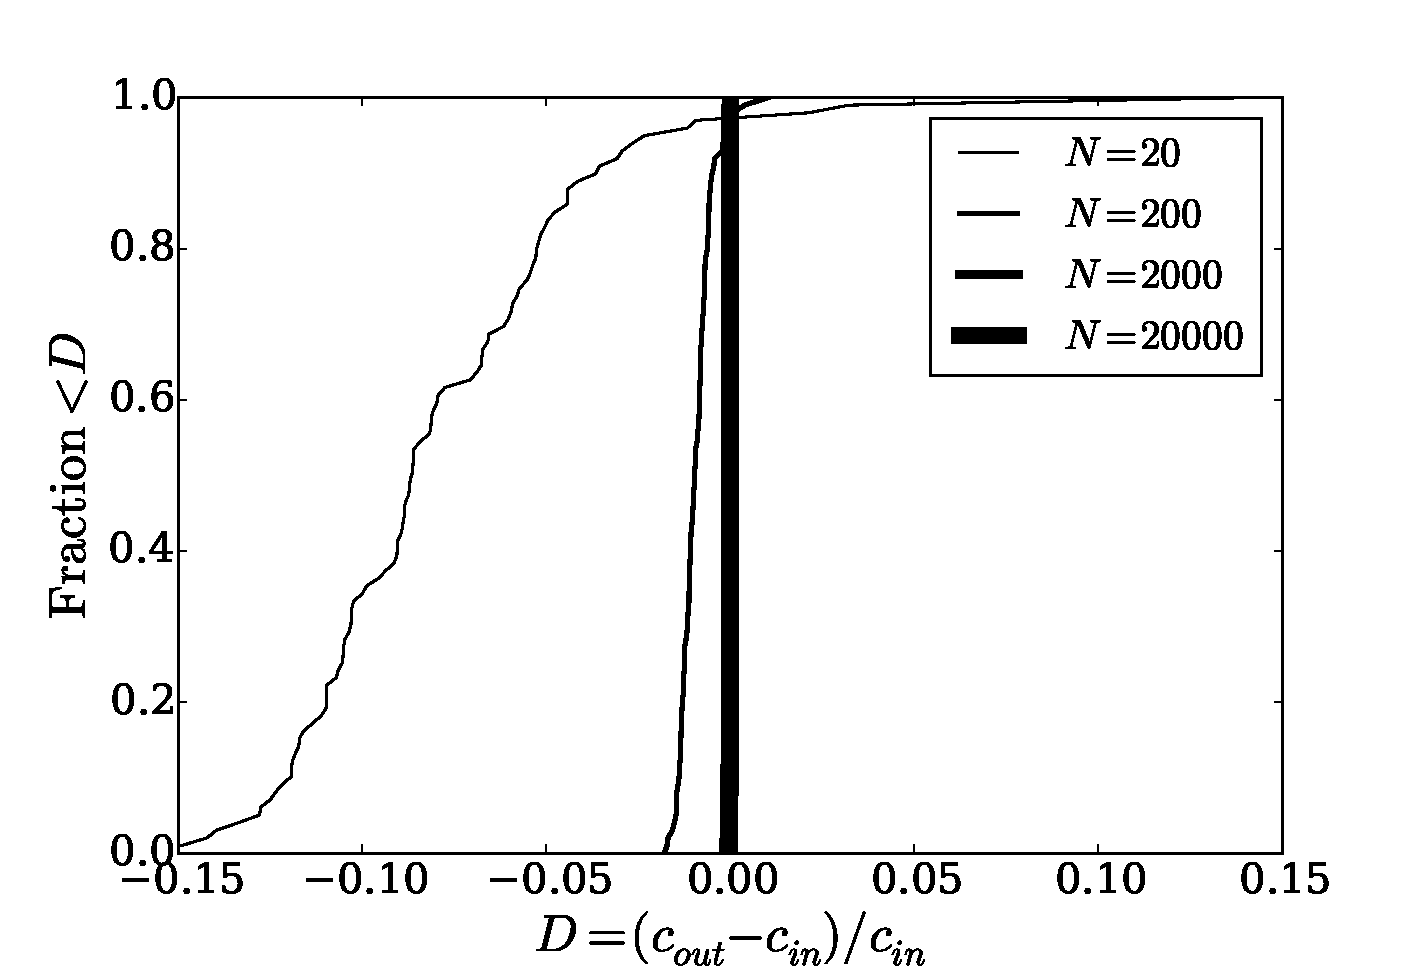
\includegraphics[width=0.50\textwidth]{mock_percentual_diff.pdf}
\end{center}
\caption{Cumulative distribution of the fractional difference, $D$, between
  the input concentration in the mock halo generator, $c_{in}$ and the
  measurement by our MCMC code, $c_{out}$. Each curve corresponds to
  halos generated with a different number of particles, $N$.
    \label{fig:results_mocks}}
\end{figure}

Figure \ref{fig:results_mocks} shows the integrated distribution for
$D$ for the fits using our method, split into four different groups
according the particle number.
From this Figure the first immediate
conclusion is that increasing the number of particles increases the
chances to recover the input values.

We believe that the main effect that contributes to this trend
is that the particle that our algorithm finds to be the halo center
(where the potential is minimum) gets closer to the original
geometrical center (where no particle sits by construction) used to
generate the halo.  Poisson noise makes this center fluctuate,
changing the numerical radial profile from the analytic input.

For particle number of $20$ the offset between the input and output
concentration can be as large as $20\%$, with a slight bias around
$-0.05\%$, i.e. the output concentration is biased towards lower
values than the input.
For particle numbers of $2000$ most of the offsets fall below $5\%$,
with a clear peak around $0\%$ indicating that any appreciable bias is
absent.


\subsubsection{The impact of the input concentration}

\begin{figure*}
  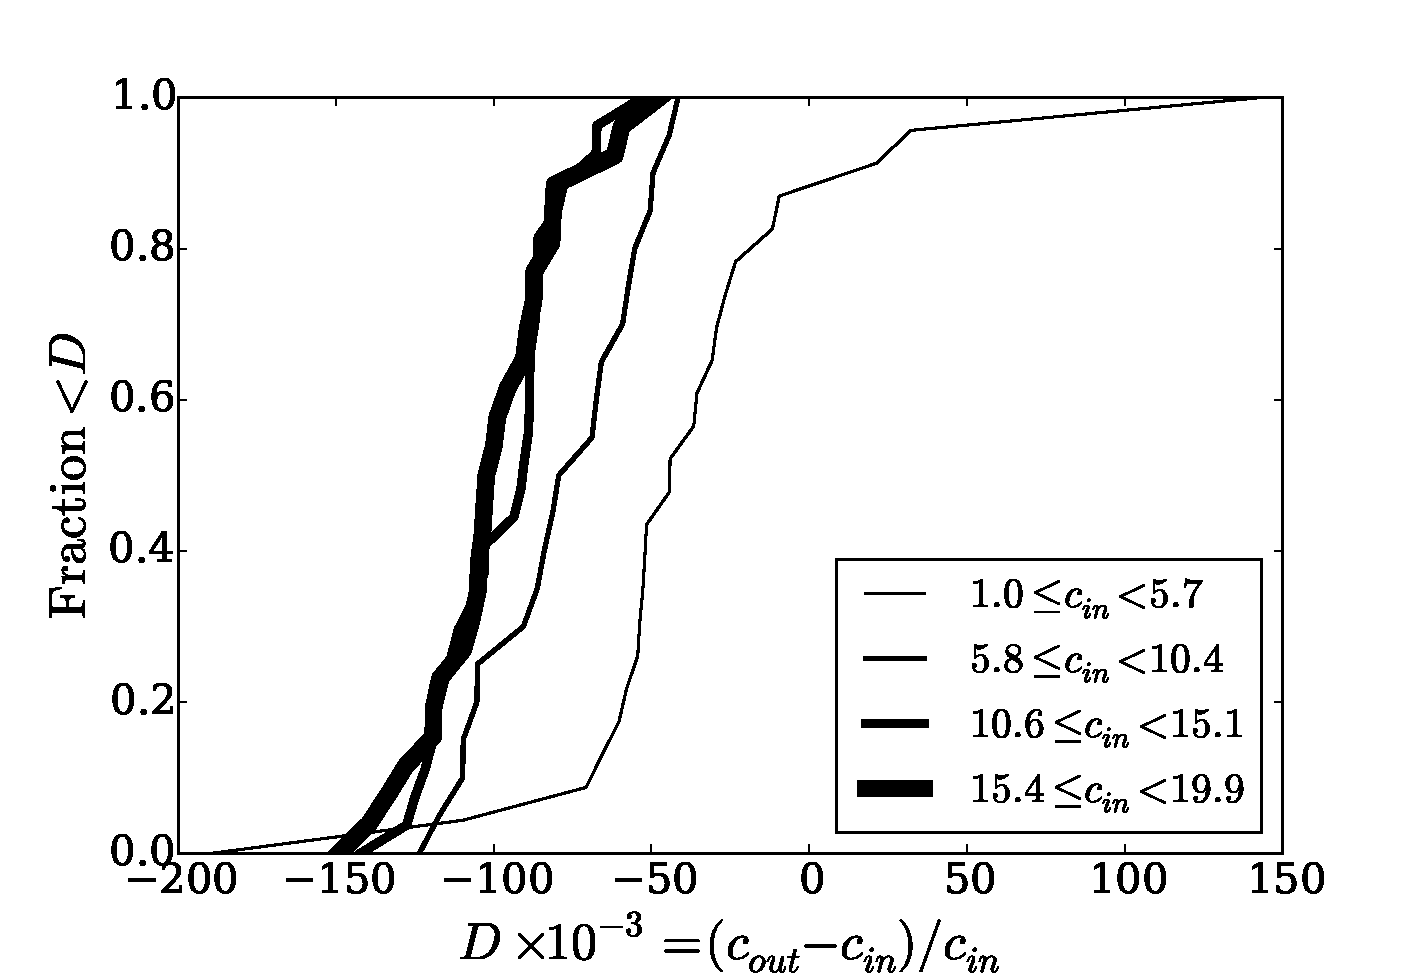
\includegraphics[width=0.45\textwidth]{mock_percentual_diff_conc_20.pdf}
  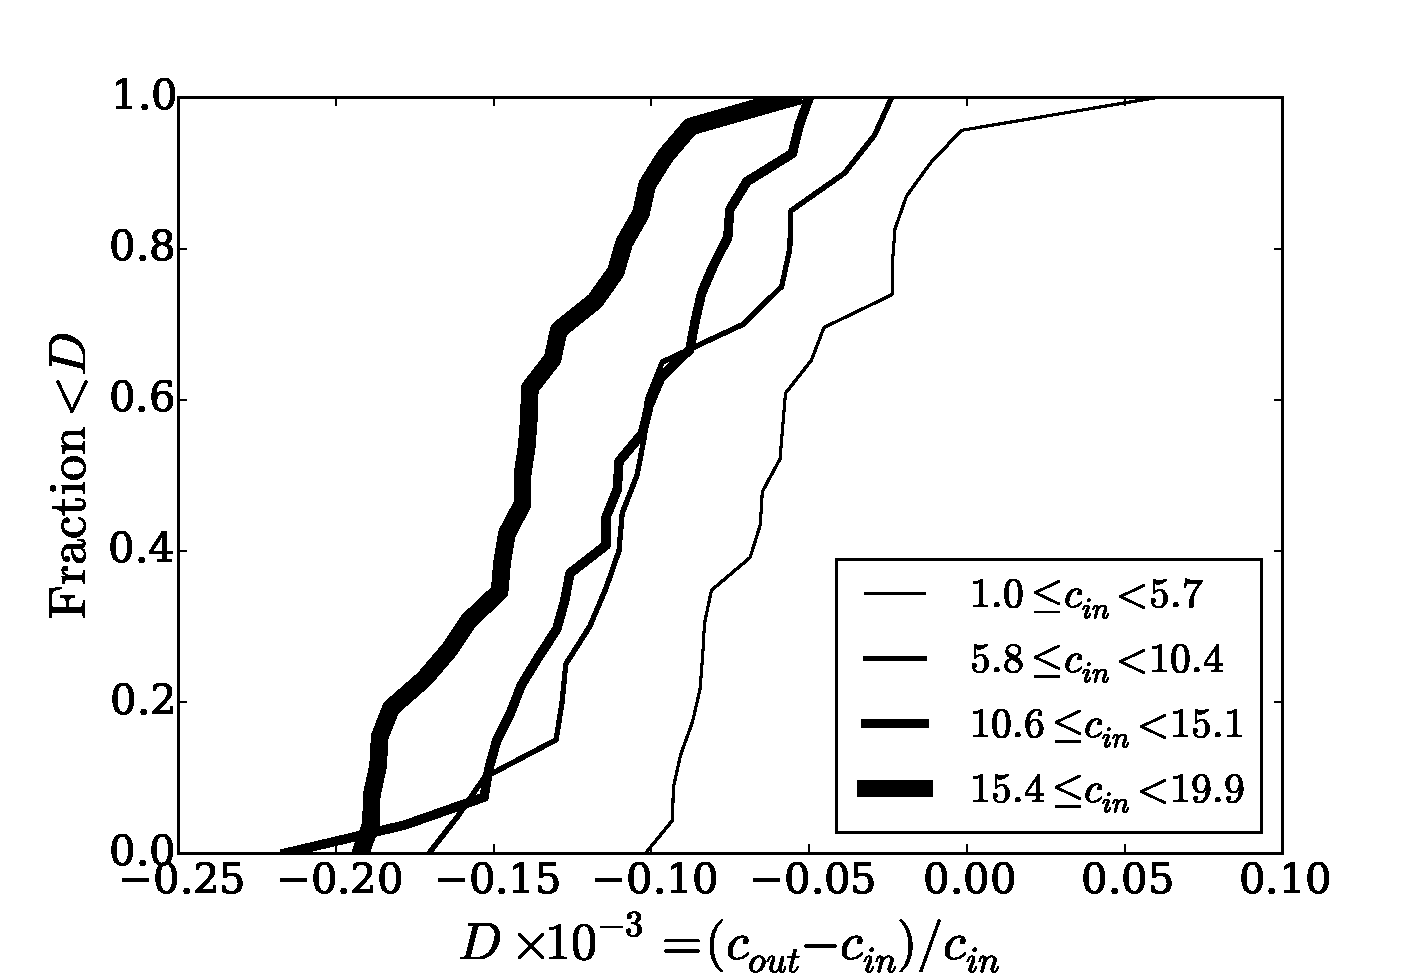
\includegraphics[width=0.45\textwidth]{mock_percentual_diff_conc_20000.pdf}
\caption{Cumulative distribution of the fractional difference, $D$, between
  the input concentration in the mock halo generator, $c_{in}$ and the
  measurement by our MCMC code, $c_{out}$. Each curve corresponds to
  halos generated with an input concentration in a different range for
  a number of particles $N=20$ (right panel) and $N=20000$ (left panel).
    \label{fig:results_mocks_conc}}
\end{figure*}

Figure \ref{fig:results_mocks_conc} shows the integrared distribution
for $D$ for the fits using our method, split into different input
concentrations for two different particle numbers describing the mock
halos. 
On the left we have the case of halos sampled with $N=20$ particles
and on the right we have show results for halos with $N=20000$
particles. 
The scale for $D$ varies by almost three orders of magnitude.
The accuracy of our method increases with larger values of $N$. 
This was already seen in the previous section. 
We explore the exact dependence of $D$ with the number of particles in
the next section when we compare the accuracy of different methods.

There are two interesting in Figure \ref{fig:results_mock_conc}. The
first is that our method tends to underestimate the concentration
and the second is that the degree of this underestimation increases
with the input halo concentration.

\subsubsection{The accuracy of different methods}

\begin{figure}
\begin{center}
  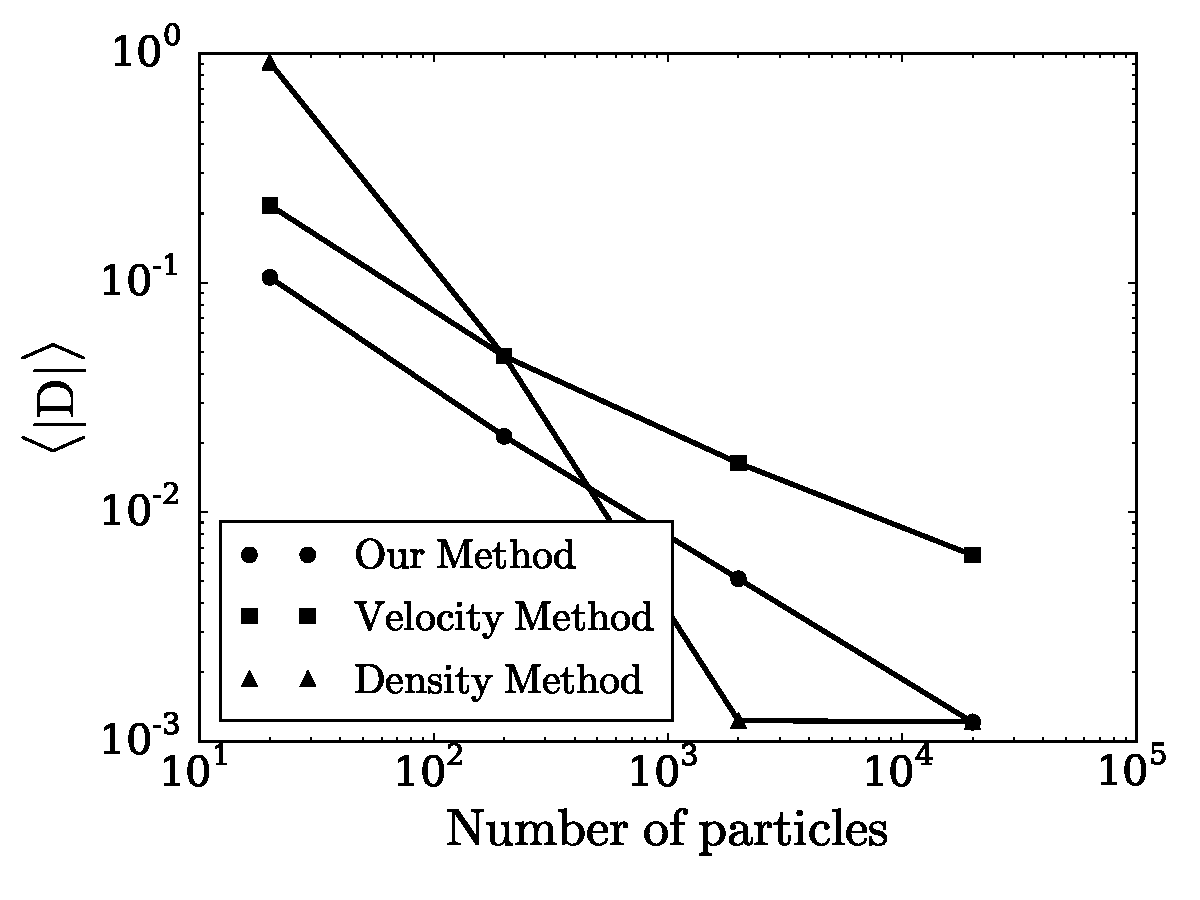
\includegraphics[width=0.48\textwidth]{error.pdf}
\end{center}
\caption{Average value of the relative error in the concentration
  estimate, $\avg{|D|}$, as a function of the particle number $N$ in
  the set of mock halos. Different symbols represent different
  methods. Our method provide the most accurate estimate at fixed
  particle number $N$.
    \label{fig:error}}
\end{figure}


Using this data-set we also compare our method against the other two
methods described earlier: using shells to estimate the density as a
function of radius and the maximum circular velocity method.
In the first case we use the same MCMC algorithm we
have in our method to fit the density profile.
In the second method we simply follow the procedure described in
Section \ref{sec:method}

We quantify the accuracy of each method with the following statistic:

\begin{equation}
\avg{|D|}=\frac{1}{\left|{\cal{H}}_N\right|}\sum_{{\cal{H}}_N} |D|,
\end{equation}
%
where ${\cal{H}}_N$ corresponds to the set of haloes with $N$
particles, $D$ follows the definition in Eq. (\ref{eq:D}) and
$\left|{\cal{H}}_n\right|$ is the number of haloes in ${\cal{H}}_n$.


Figure \ref{fig:error} shows the behaviour of $\avg{|D|}$ as a function of
halo particle number for the three different methods to estimate the
concentration.

At fixed particle numbers our method almost always shows the lowest
$\avg{|D|}$ values compared to the other two methods.
Its accuracy is on the order of $10\%$ for $20$ particles in the halo,
going down to $0.1\%$ for halos with $20000$ particles.
The decrease of $\avg{|D|}$ with increasing particle number $N$ goes
approximately as $\avg{|D|}\propto N^{-1/2}$, which reinforces the hint that
the accuracy of the method is related to a decrease of Poisson
noise.

The method based on the maximum of the circular velocity shows a similar
behaviour $\avg{|D|}\propto N^{-1/2}$. Its accuracy is $2-5$ times less
than in our method, on the order of $20\%$ for $20$ particle halos and
$0.5\%$ for $20000$ particle halos. The method based on the direct density
fit shows the lowest accuracy for a low particle number and an intermediate
accuracy between the other two methods for a high particle number.

\subsection{Tests on N-body data}
\label{sec:data}
\begin{figure*}
  \begin{center}
    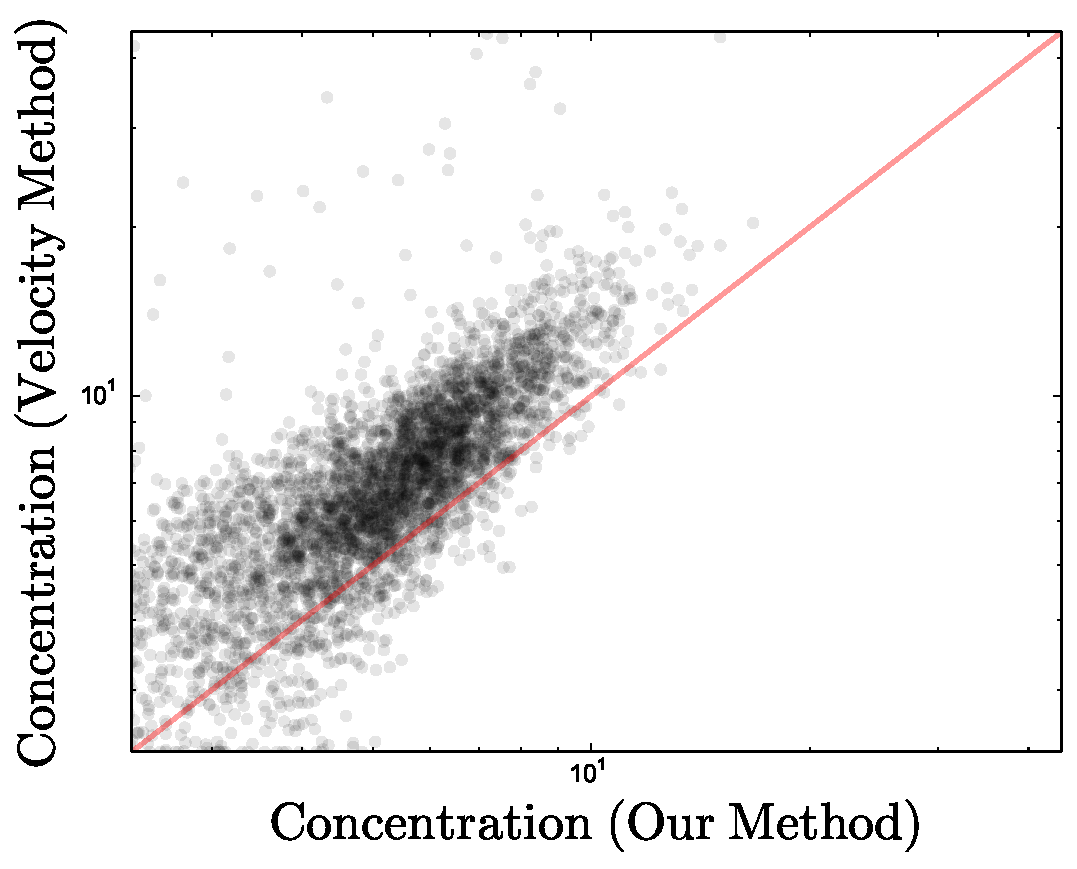
\includegraphics[width=0.33\textwidth]{mass-velocity.pdf}
    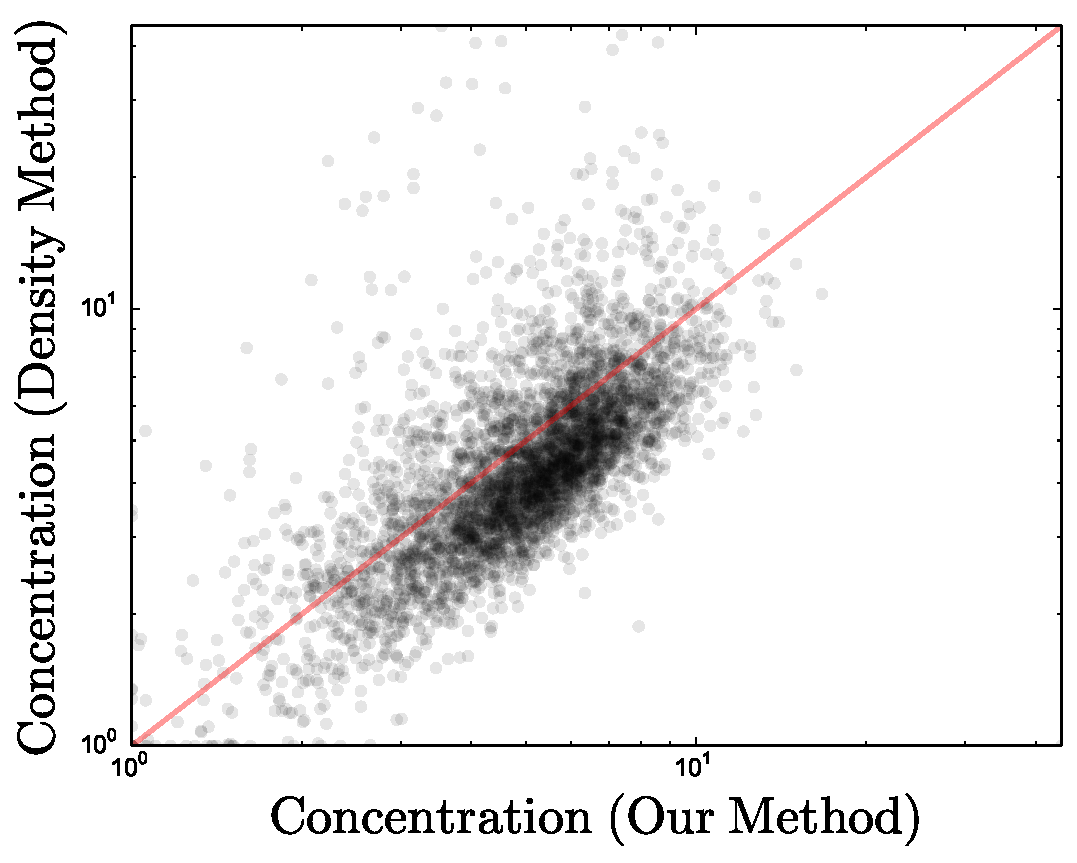
\includegraphics[width=0.33\textwidth]{mass-density.pdf}
    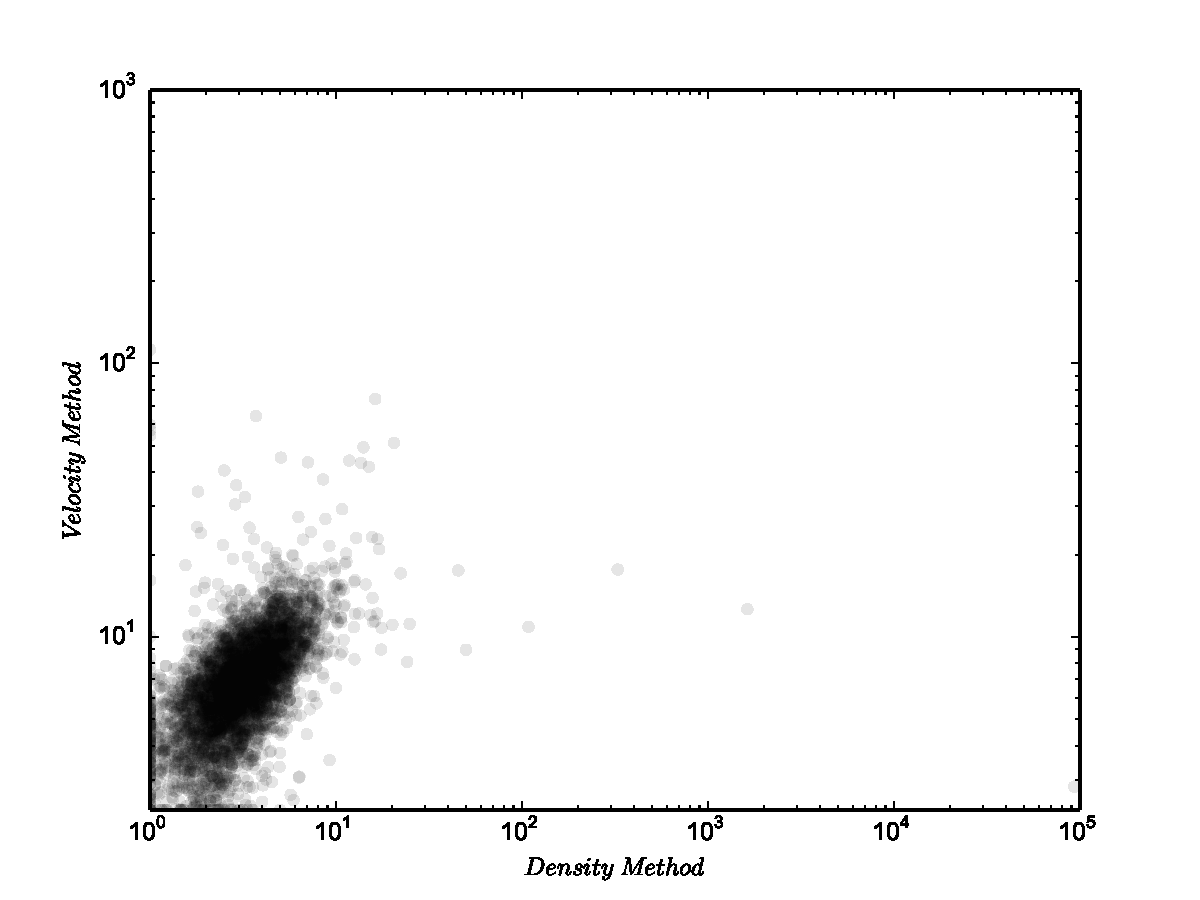
\includegraphics[width=0.33\textwidth]{density-velocity.pdf}
  \end{center}
  \caption{Comparison between the concentrations measured by our
    method and the maximum velocity (left) and density (middle)
    methods. The line indicates the equal value between the two
    techniques. The right panel compares the results of the maximum
    velocity and density methods.
  \label{fig:mdv}}
\end{figure*}

We use data from a N-body cosmological simulation that follows the non
non-linear evolution of a dark matter density field sampled with
$512^3$ particles over a cubic box of $400$ \hMpc on a side. 
This simulation was run with the public available version of the
Gadget-2 code. 
The simulation uses a standard $\Lambda$CDM cosmology with values of
$\Omega_m=0.258$, $\Omega_\Lambda=0.742$ and $h=0.72$ for the matter
density parameter, cosmological constant parameter and the reduce
Hubble constant, respectively. 
With these parameters the mass of an individual simulation particle
corresponds to $3.41\times 10^{10}$\hMsun.

{\bf descripcion del halo finder}

{\bf descripcionde separacion por grado de relajacion}.


{\bf describcion de los resultados}
Figure \ref{fig:mdv} shows the results that compare the concentration
values in the simulated halos from the three different methods.



\begin{figure*}
\begin{center}
  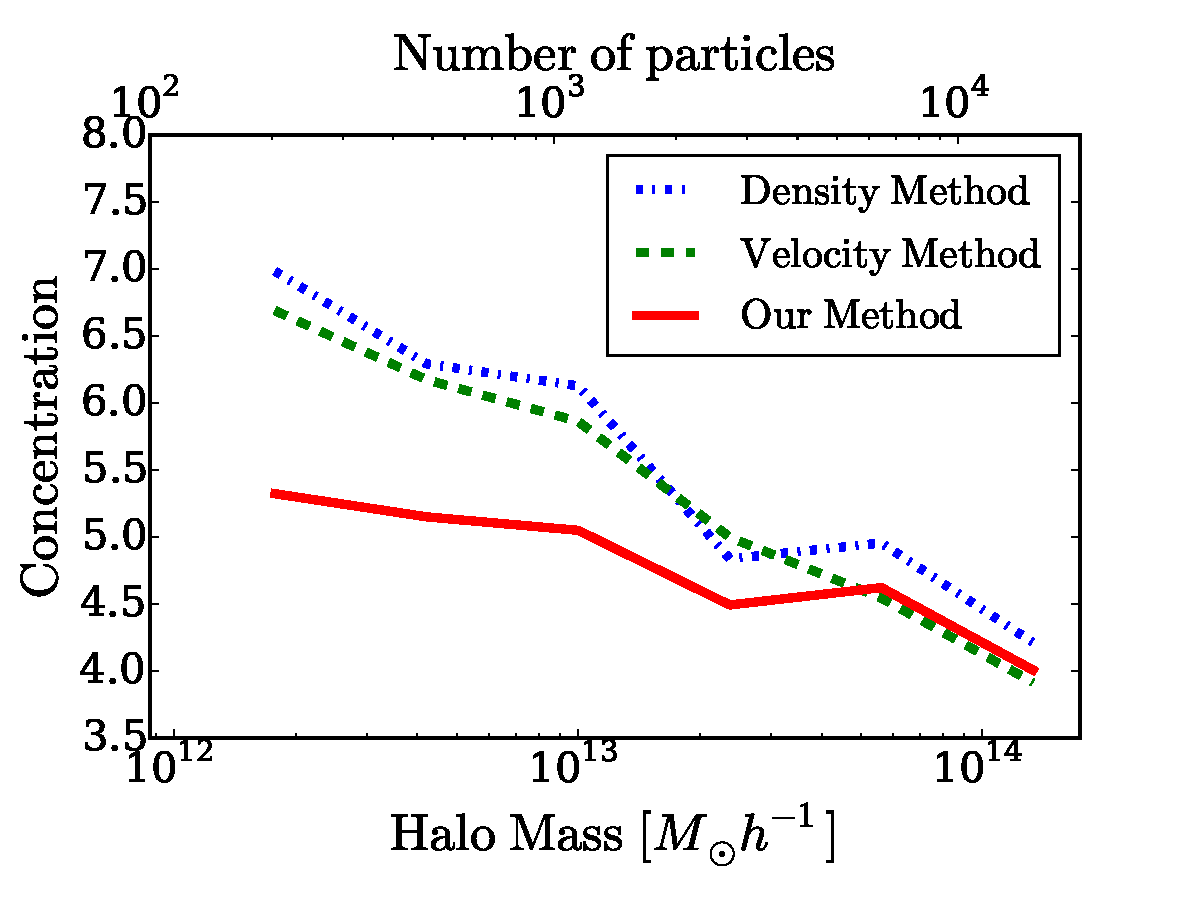
\includegraphics[width=0.90\textwidth]{concentration.pdf}
\end{center}
\caption{Mass-concentration relationship for the three different
  methods used on the same cosmological N-body data. The central lines
  correspond the median and the shadowed region indicates the
  quartiles.
    \label{fig:concentration}}
\end{figure*}




\section{Conclusions}
\label{sec:conclusions}

In this paper, we presented a new method to estimate the
concentration of dark matter halos in N-body simulations. 
We tested our method on mock halo data to study the impact of total
number of particles and input concentration on the retrieved values.
We compared these results against two other methods commonly used in
the literature to estimate concentrations.
Finally, we applied our method to halos extracted from a cosmological
N-body simulation to estimate the impact of our method on the mass
concentration relationship. 

Comparison against other methods.\\

The effect of the number of particles.\\

The effect of the input concentration.\\

The impact on the mass-concentration relationship.\\

Comment and future.\\



\bibliography{references}

\end{document}
